\documentclass[11pt]{article}
\usepackage{preamble}
\titleformat*{\section}{\Large\bfseries}
\usepackage{mathtools}
\usepackage{listings, courier}
\lstset{basicstyle=\small\ttfamily,breaklines=true}
\lstset{
      numbers=left,
      stepnumber=1,    
      firstnumber=1,
      numberfirstline=true,
      xleftmargin=6em,
      framexleftmargin=3.5em,
      framextopmargin=6pt,
      framexbottommargin=6pt, 
      frame=tb, framerule=0pt,  
      numberstyle=\small\color{gray},
      numbersep=20pt,
      backgroundcolor=\color{gray!10},
}
\DeclarePairedDelimiter\ceil{\lceil}{\rceil}
\DeclarePairedDelimiter\floor{\lfloor}{\rfloor}
\def\columnseprulecolor{\color{blue}}

\title{CISC 3220 Homework Chapter 15}
\author{Rachel Friedman}
\date{May 10, 2020}

\begin{document}
\maketitle

\section*{Exercises 15.2}\nointerlineskip
\noindent \rule{\linewidth}{0.01pt}\\

\subsubsection*{Question 15.2-1}\nointerlineskip
Find an optimal parenthesization of a matrix-chain product whose sequence of dimensions is $\langle 5, 10, 3, 12, 5, 50, 6 \rangle$.\\

An optimal parenthesization of that sequence is $(A_1 A_2)((A_3 A_4)(A_5 A_6))$ as shown below:\\

$(A_1 A_2)$ = 5 x 10 x 3 = 150 operations, resulting in a 5 x 3 matrix\\
\indent $(A_3 A_4)$ = 3 x 12 x 5 = 180, resulting in a 3 x 5 matrix\\
\indent $(A_5 A_6)$ = 5 x 50 x 6 = 1500, resulting in a 5 x 6 matrix\\
\indent $(A_3 A_4)(A_5 A_6)$ = 3 x 5 x 6 = 90, resulting in a 3 x 6 matrix\\
\indent $(A_1 A_2)  ((A_3 A_4)(A_5 A_6))$ = 5 x 3 x 6 = 90.\\

Total operations = 150 + 180 + 1500 + 90 + 90 = 2100.\\

\section*{Exercises 15.4}\nointerlineskip
\noindent \rule{\linewidth}{0.01pt}\\
\subsubsection*{Question 15.4-1}\nointerlineskip
Determine an LCS of $\langle$ 1, 0, 0, 1, 0, 1, 0, 1 $\rangle$ and $\langle$ 0, 1, 0, 1, 1, 0, 1, 1, 0 $\rangle$⟩.\\
Answer: $\langle$ 1, 0, 0, 1, 1, 0 $\rangle$\\
\begin{center}
\includegraphics[scale=.4]{ques_LCS.png}
\end{center}

\subsubsection*{Question 15.4-2}\nointerlineskip
Give pseudocode to reconstruct an LCS from the completed $c$ table and the original sequences $X = \langle$ ....$\rangle$ and $Y = \langle$ ....$\rangle$, without using the $b$ table.\\

\begin{minipage}{6in}
\begin{lstlisting}[language=Python]
PRINT-LCS(c, X, Y, i, j)
    if c[i, j] == 0
        return
    if X[i] == Y[j]
        PRINT-LCS(c, X, Y, i - 1, j - 1)
        print X[i]
    else if c[i - 1, j] > c[i, j - 1]
        PRINT-LCS(c, X, Y, i - 1, j)
    else
        PRINT-LCS(c, X, Y, i, j - 1)
    
\end{lstlisting}
\end{minipage}

\section*{Exercises 15.5}\nointerlineskip
\noindent \rule{\linewidth}{0.01pt}\\

\subsubsection*{Question 15.5-1}\nointerlineskip
Write pseudocode for the procedure CONSTRUCT-OPTIMAL-BST.root which,
given the table root, outputs the structure of an optimal binary search tree.\\

\begin{minipage}{6in}
\begin{lstlisting}[language=Python]
CONSTRUCT-OPTIMAL-BST(root, i, j, last)
    if i == j
        return
    if last == 0
        print root[i, j] + "is the root"
    else if j < last:
        print root[i, j] + "is the left child of" + last
    else
        print root[i, j] + "is the right child of" + last
    CONSTRUCT-OPTIMAL-BST(root, i, root[i, j] - 1, root[i, j])
    CONSTRUCT-OPTIMAL-BST(root, root[i, j] + 1, j, root[i, j])
\end{lstlisting}
\end{minipage}

\subsubsection*{Question 15.5-2}\nointerlineskip
Determine the cost and structure of an optimal binary search tree for a set of $n=7$
keys with the following probabilities:\\
\begin{center}
\begin{tabular}{c | c c c c c c c c}
i & 0 & 1 & 2 & 3 & 4 & 5 & 6 & 7 \\ 
\hline
$p_i$ &  & .04 & .06 & .08 & .02 & .10 & .12 & .14 \\
$q_i$ & .06 & .06 & .06 & .05 & .05 & .05 & .05 & .05 \\   
\end{tabular}
\end{center}

\begin{center}
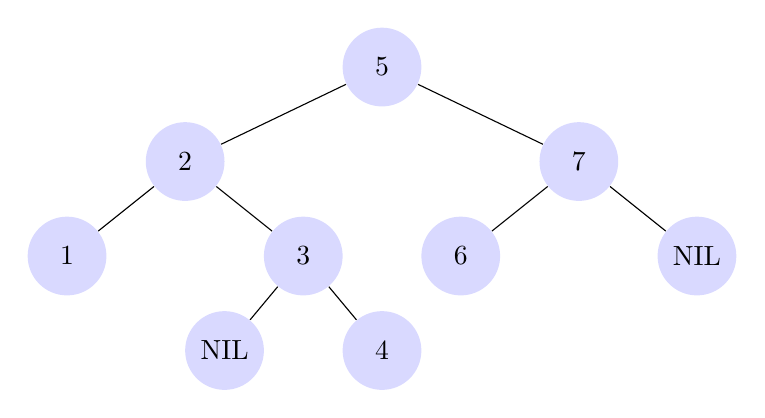
\begin{tikzpicture}
  [level distance = 12mm, node distance=0.1,
   every node/.style={fill=blue!15!white,circle, inner sep=1pt, minimum size=10mm},
   level 1/.style={sibling distance = 50mm},
   level 2/.style={sibling distance = 30mm},
   level 3/.style={sibling distance = 20mm},
   level 3/.style={sibling distance = 20mm}]

  \node {5}
     child {node{2}
       child {node {1}}
       child {node {3}
        child {node {NIL}}
        child {node {4}}
       }
     }
     child {node{7}
       child {node {6}}
       child {node {NIL}}
     };
\end{tikzpicture}
\end{center}
(For simplification purposes, I eliminated the dummy variables.)\\
Cost of optimal binary search tree = 3.12.\\

\end{document}